\subsection{Sensitivity analysis figures:}
\subsubsection{Short term}
\begin{figure} [H]
    \centering
    \caption{Positive news: event identification rule}
    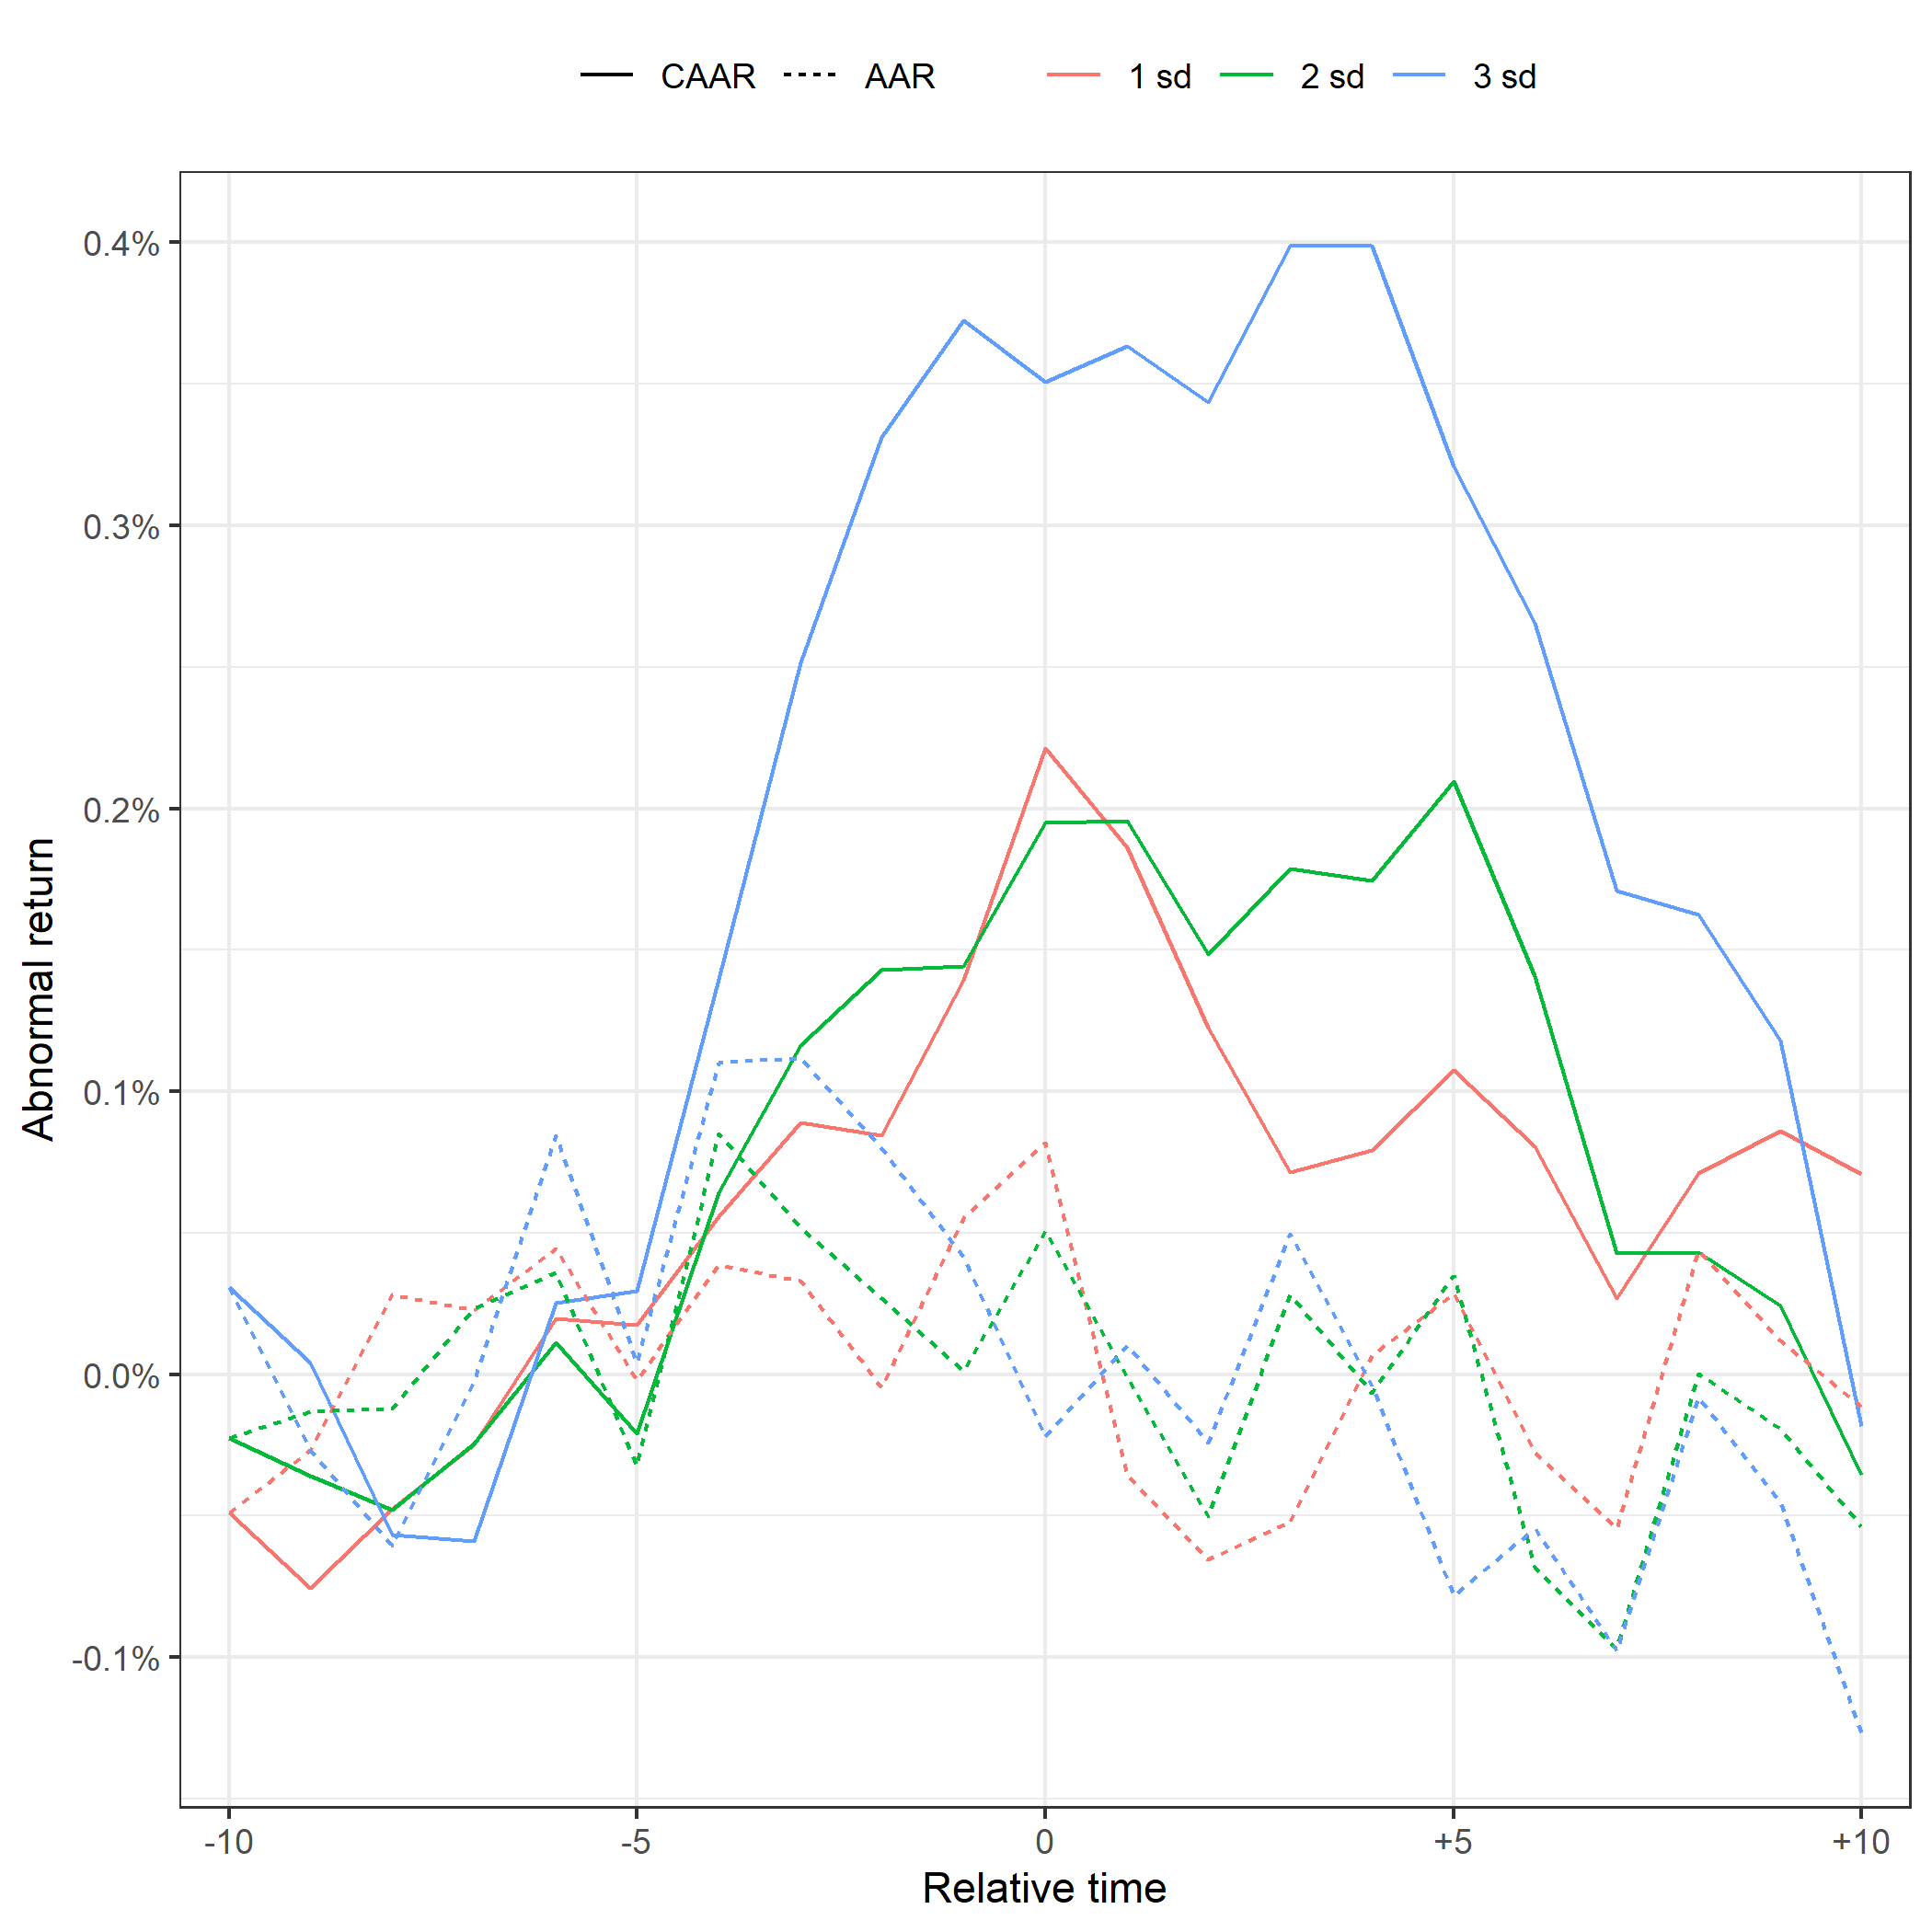
\includegraphics[scale=0.6]{Projekt/1.Figures analysis/ST_positive_sensitivity.png}
     \caption*{\footnotesize The figure illustrates the average abnormal return (AAR) and cumulative AAR (CAAR) around the event date (t = 0) of negative news. The figure illustrates the average abnormal return (AAR) and cumulative AAR (CAAR) around the event date (t = 0) of negative news. The various colors represent whether the event identification rule was based on 1, 2, or 3 standard errors. }
    \label{fig:ST_pos_sensi_sd}
\end{figure} 

\begin{figure} [H]
    \centering
    \caption{Positive news: Value vs. Equal weights}
    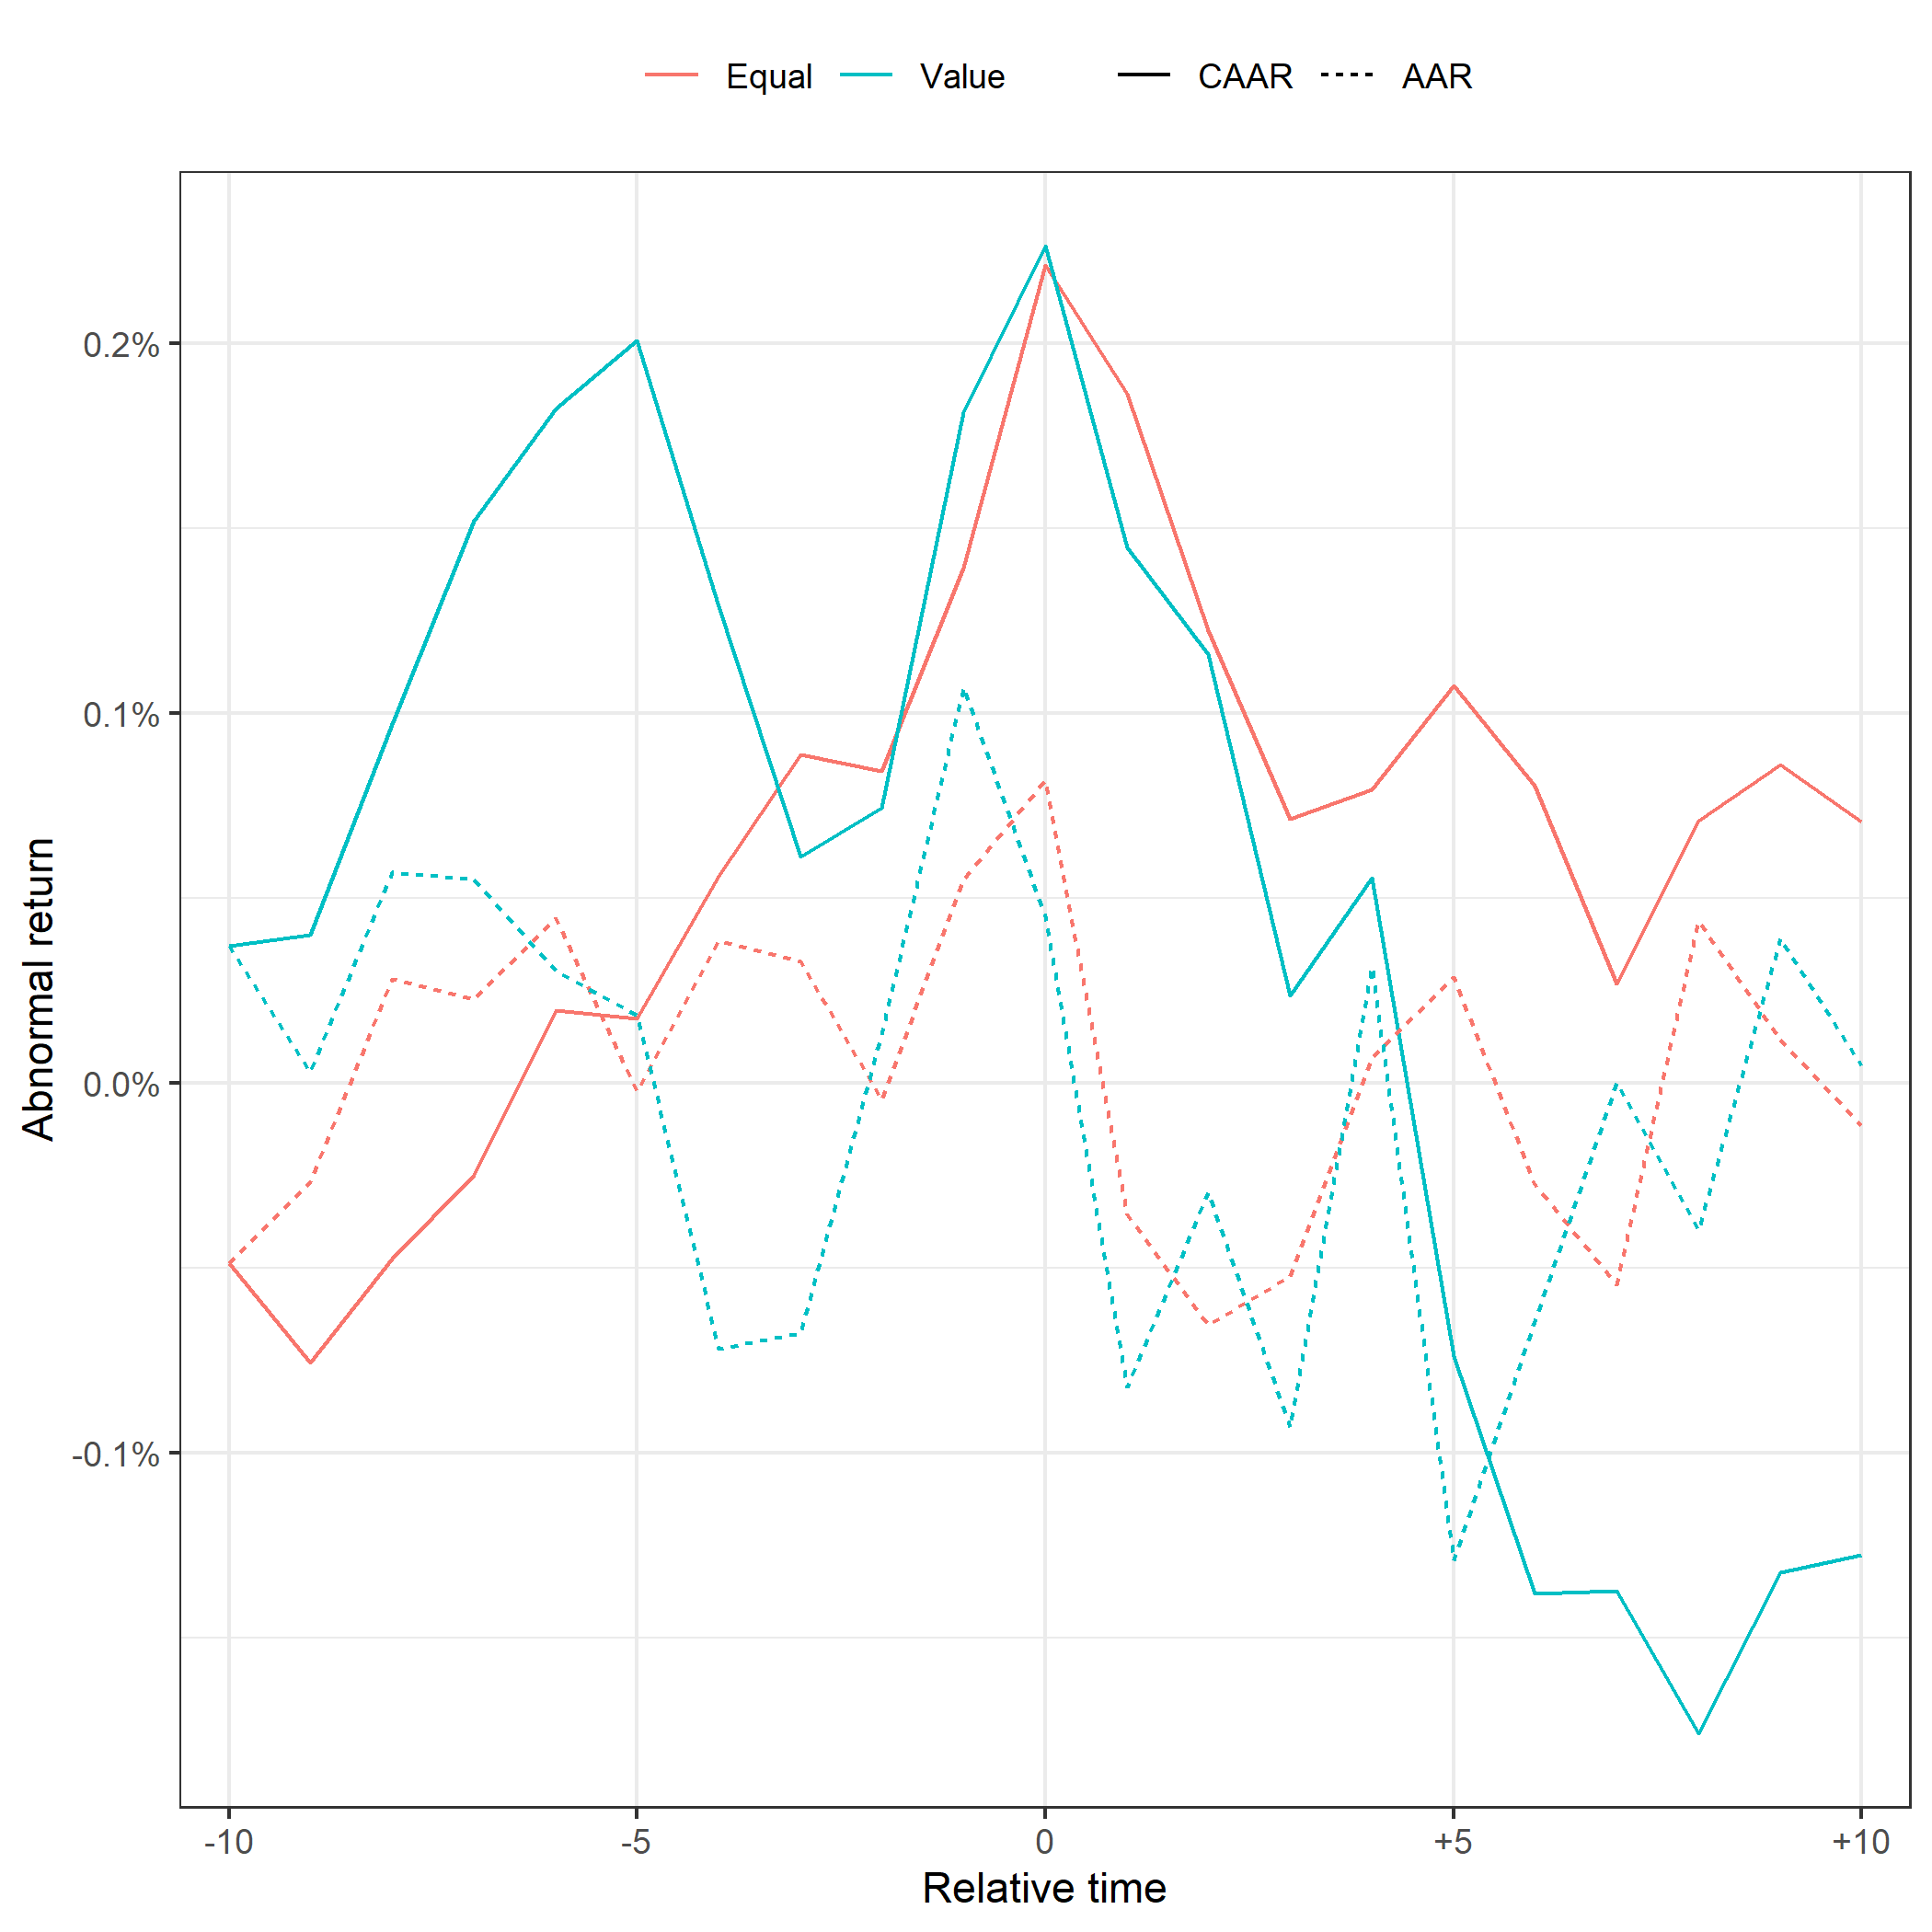
\includegraphics[scale=0.6]{Projekt/1.Figures analysis/ST_positive_sensitivity_weight.png}
     \caption*{\footnotesize The figure illustrates the average abnormal return (AAR) and cumulative AAR (CAAR) around the event date (t = 0) of positive news. The blue lines are returns calculated from an equally weighted portfolio, while the weights of the red lines are based on market capitalization. }
    \label{fig:ST_pos_sensitivity_weights}
\end{figure} 

\subsubsection{Long term}


\setlength{\tabcolsep}{15pt}
\begin{table}[]
\small
\centering
\caption{Fama-French five-factor model alpha from positive news with equal weights} 
\begin{tabular}{ccccccc}
\hline \hline \\ 
 &     &  &    1 SD  &  2 SD  &  3 SD  &  \\ \cline{4-6} 
& & & \multicolumn{3}{c}{ T = 1} & \\ \cline{2-6}
& Alpha (\%)  &  & $ -0.004$  & $-0.000$  & $-0.006$ &  \\
& t-value &  & -1.55 & -0.27  & -1.48 & \\
& & & \multicolumn{3}{c}{ T = 4} & \\ \cline{2-6}
& Alpha (\%)  &  & $ -0.003^{*}$  & $-0.001^{***}$  &  $-005^{**}$ & \\
& t-value & & -1.77  & -0.75 & -227 & \\
& & & \multicolumn{3}{c}{ T = 8} & \\ \cline{2-6}
& Alpha (\%)  &  & $ -0.003^{***}$   & $-0.003^{**}$  & $-0.005^{**}$ &  \\
& t-value &  & -2.98  & -2.45 & 3.51 & \\
&  & & \multicolumn{3}{c}{ T = 12} & \\ \cline{2-6}
& Alpha (\%)  &  & $ -0.004^{***}$  & $-0.003^{**}$  & $-0.003^{**}$ &  \\
& t-value &  & -3.02  & -2.66 & -1.12 & \\
\hline \hline
 \multicolumn{7}{l}{ \footnotesize $^* \; p\; <\; 0.1$, $ ^{**} \; p\; <\; 0.05$, $ ^{***} \; p\; <\; 0.01$  } \\
 \multicolumn{7}{p{11.5cm}}{ \footnotesize Alpha is the WLS-regression intercept (in \%) of the Fama-French 3-factor model, displayed along with the corresponding t-value. N is the average amount of firms included in the portfolio each month, and T is the portfolio holding period. The threshold for event firms to be included in the portfolio is either 1,2 or 3 "SD" (standard deviations) larger than the mean.}  \\ 
\end{tabular}
\label{tab: FF5_pos_equalW}
\end{table}


\setlength{\tabcolsep}{15pt}
\begin{table}[]
\small
\centering
\caption{Fama-French five-factor model alpha from positive news with RF = 0} 
\begin{tabular}{ccccccc}
\hline \hline \\ 
 &     &  &    1 SD  &  2 SD  &  3 SD  &  \\ \cline{4-6} 
& & & \multicolumn{3}{c}{ T = 1} & \\ \cline{2-6}
& Alpha (\%)  &  & $-0.28$  & $0.02$  & $-0.38$ &  \\
& t-value &  & -1.08 & -0.06  & -0.78 & \\
& & & \multicolumn{3}{c}{ T = 4} & \\ \cline{2-6}
& Alpha (\%)  &  & $ -0.004$  & $-0.02$  &  $-0.08$ & \\
& t-value & & -0.28  & 0.11 & --0.26 & \\
& & & \multicolumn{3}{c}{ T = 8} & \\ \cline{2-6}
& Alpha (\%)  &  & $ -0.00$   & $-0.003^{**}$  & $0.03$ &  \\
& t-value &  & 0.05  & -0.17 & 0.16 & \\
&  & & \multicolumn{3}{c}{ T = 12} & \\ \cline{2-6}
& Alpha (\%)  &  & $ -0.05$  & $0.13$  & $0.23$ &  \\
& t-value &  & 0.77  & 1.06 & 1.32 & \\
\hline \hline
 \multicolumn{7}{l}{ \footnotesize $^* \; p\; <\; 0.1$, $ ^{**} \; p\; <\; 0.05$, $ ^{***} \; p\; <\; 0.01$  } \\
 \multicolumn{7}{p{11.5cm}}{ \footnotesize Alpha is the WLS-regression intercept (in \%) of the Fama-French 3-factor model, displayed along with the corresponding t-value. N is the average amount of firms included in the portfolio each month, and T is the portfolio holding period. The threshold for event firms to be included in the portfolio is either 1,2 or 3 "SD" (standard deviations) larger than the mean.}  \\ 
\end{tabular}
\label{tab: FF5_RF}
\end{table}

